%% abtex2-modelo-slides.tex, v-1.0 gfabinhomat
%% Copyright 2012-2018 by abnTeX2 group at http://www.abntex.net.br/ 
%%
%% This work may be distributed and/or modified under the
%% conditions of the LaTeX Project Public License, either version 1.3
%% of this license or (at your option) any later version.
%% The latest version of this license is in
%%   http://www.latex-project.org/lppl.txt
%% and version 1.3 or later is part of all distributions of LaTeX
%% version 2005/12/01 or later.
%%
%% This work has the LPPL maintenance status `maintained'.
%% 
%% The Current Maintainer of this work is Fábio Rodrigues Silva, 
%% member of abnTeX2 team, led by Lauro César Araujo. 
%% Further information are available on 
%% http://www.abntex.net.br/
%%
%% This work consists of the files abntex2-modelo-slides.tex, 
%% abntex2-modelo-references.bib and abntex2-modelo-marca.pdf
%%
%% Modelo desenvolvido por Fábio Rodrigues Silva (gfabinhomat@gmail.com)
%% Mais informações podem ser obtidas no guia do usuário Beamer 
%% (http://linorg.usp.br/CTAN/macros/latex/contrib/beamer/doc/beameruserguide.pdf)
%% Informações rápidas podem ser acessadas em http://en.wikibooks.org/wiki/LaTeX/Presentations


% Apresentações em widescreen. Outros valores possíveis: 1610, 149, 54, 43 e 32.
% Por padrão, as apresentações são no formato 4:3 (sem o aspectratio).
\documentclass[aspectratio=169]{beamer}	 	

\usetheme{Pittsburgh}
\usecolortheme{default}
\usefonttheme[onlymath]{serif}			% para fontes matemáticas
% Enconte mais temas e cores em http://www.hartwork.org/beamer-theme-matrix/ 
% Veja também http://deic.uab.es/~iblanes/beamer_gallery/index.html

% Customizações de Cores: fg significa cor do texto e bg é cor do fundo
\setbeamercolor{normal text}{fg=black}
\setbeamercolor{alerted text}{fg=red}
\setbeamercolor{author}{fg=blue}
\setbeamercolor{institute}{fg=blue}
\setbeamercolor{date}{fg=green}
\setbeamercolor{frametitle}{fg=red}
\setbeamercolor{framesubtitle}{fg=brown}
\setbeamercolor{block title}{bg=blue, fg=white}		%Cor do título
\setbeamercolor{block body}{bg=lightgray, fg=darkgray}	%Cor do texto (bg= fundo; fg=texto)

% ---
% PACOTES
% ---
\usepackage{ragged2e}
\usepackage[alf, abnt-emphasize=bf]{abntex2cite}	 % Citações padrão ABNT
\usepackage[brazil]{babel}		% Idioma do documento
\usepackage{color}			% Controle das cores
\usepackage[T1]{fontenc}		% Selecao de codigos de fonte.
\usepackage{graphicx}			% Inclusão de gráficos
\usepackage[utf8]{inputenc}		% Codificacao do documento (conversão automática dos acentos)
\usepackage{txfonts}			% Fontes virtuais
\usepackage{multimedia}
\usepackage{float}
\usepackage{unicode-math}
\usepackage{amsmath}
\usepackage{siunitx}
% ---

\graphicspath{{IMAGENS}{PDF}}

\newcounter{saveenumi}
\newcommand{\seti}{\setcounter{saveenumi}{\value{enumi}}}
\newcommand{\conti}{\setcounter{enumi}{\value{saveenumi}}}

\resetcounteronoverlays{saveenumi}

% --- Informações do documento ---
\title{Sistema Operacional Embarcado \\ NuttX\footnote[frame]{\cite{nuttx}}}
\author{Gustavo Vianna França}
\date{\today}
% ---

\AtBeginSection[]
{
    \begin{frame}
        \frametitle{Sumário}
        \tableofcontents[currentsection]
    \end{frame}
}

% ----------------- INÍCIO DO DOCUMENTO --------------------------------------
\begin{document}

% ----------------- NOVO SLIDE --------------------------------
\begin{frame}

\begin{minipage}{1\linewidth}
  \centering
  \begin{tabular}{cc}
    \begin{tabular}{c}
      
\includegraphics[width=3.0cm]{florianopolis_horizontal_marca2015.pdf}
    \end{tabular}
    &
    \begin{tabular}{c}
      
\includegraphics[width=0.45\textwidth]{daeln_horizontal.pdf}
    \end{tabular}
  \end{tabular}
\end{minipage}

\titlepage

\end{frame}

% ----------------- NOVO SLIDE --------------------------------
\begin{frame}{Sumário}
\tableofcontents
\end{frame}

% ----------------- NOVO SLIDE --------------------------------
\section{Introdução}
\begin{frame}{Introdução}

\begin{minipage}{0.5\textwidth}
  \begin{itemize}
    \justifying
    \item \visible<1->{Criado por Gregory Nutt\footnote[frame]{\cite{nutt}}, experiente desenvolvedor de sistemas embarcados no campo aeroespacial, também criou os sistemas utilizados nas impressoras HP;}
    \item \visible<2->{NuttX é um sistema operacional com suporte a tempo real direcionado para microcontroladores e dispositivos IoT;}
    \item \visible<3->{\textit{Software} de código aberto e gratuito, licenciado de forma permissiva por meio da Apache \textit{Licence} 2.0, no que ele pertence à incubadora da Apache \textit{Software Foundation}.}
  \end{itemize}
\end{minipage}%
\begin{minipage}{0.5\textwidth}
  \centering
  \begin{overprint}
  	\onslide<1>\centering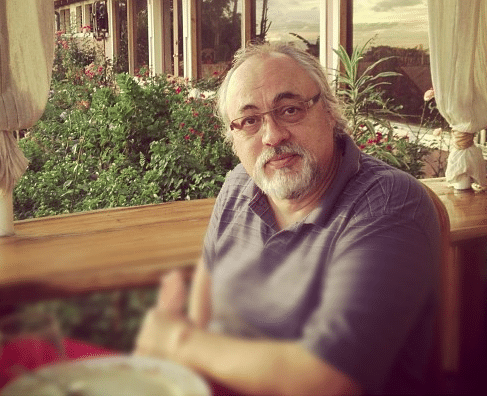
\includegraphics[width=0.95\linewidth]{nutt.png}
	\onslide<2>\centering
\includegraphics[width=0.5\linewidth]{NuttX.png}
	\onslide<3>\centering
\includegraphics[width=0.95\linewidth]{Apache.png}
  \end{overprint}
\end{minipage}

\end{frame}

% ----------------- NOVO SLIDE --------------------------------
\section{Funcionalidades}
\begin{frame}{Funcionalidades}
\framesubtitle{Principais}

\begin{itemize}
	\justifying
	\item \visible<1->{Segue de maneira rígida os padrões \textit{Portable Standard OS Interface} (POSIX) e \textit{American National Standards Institute} (ANSI);}
	\item \visible<2->{Escrito quase exclusivamente em C e é escalável para microcontroladores de 8-bit a 64-bit;}
	\item \visible<3->{Design modular e configurável;}
	\item \visible<4->{Possui gerenciamento de tarefas, com suporte a preempção, a operação \textit{tickless} e a \textit{Inter-Process Communication} (IPC).}
\end{itemize}

\end{frame}

% ----------------- NOVO SLIDE --------------------------------
\begin{frame}{Funcionalidades}
\framesubtitle{Plataformas}

\begin{minipage}{0.5\textwidth}
	\begin{itemize}
		\justifying
		\item Suporta microcontroladores com arquitetura ARM (Famílias Cortex-A, Cortex-M, e outros)\footnote[frame]{\cite{wiki}};
		\item RISC-V (SiFive FE310, Espressif Systems ESP32-C3, Kendryte K210 e outros);
		\item AVR (ATmega, AT90USB e AVR32);
		\item MIPS (PIC32MX e PIC32MZ);
		\item Zilog, Xtensa, Intel, OpenRISC e Renesas/Hitachi.
	\end{itemize}
\end{minipage}%
\begin{minipage}{0.5\textwidth}
  \centering
  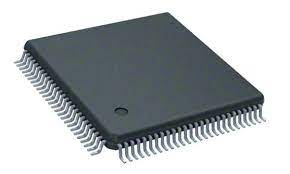
\includegraphics[width=0.95\linewidth]{microcontrolador.jpg}
\end{minipage}

\end{frame}

% ----------------- NOVO SLIDE --------------------------------
\begin{frame}{Funcionalidades}
\framesubtitle{Outras}

\begin{itemize}
	\justifying
	\item Sistemas de arquivos \textit{Virtual File System} (VFS), FAT 12/16/32, \textit{Network File System} (NFS), suporte para cartões de memória
	que comunicam por SPI como \textit{MultiMediaCard} (MMC) e \textit{Secure Digital} (SD/SDHC) e outros;
	\item Camada de rede que suporta TCP/IP, UDP, ICMP, IGMP, DNS, camada de \textit{sockets} (compatível com BSD) e utilitários como DHCP, SMTP, FTP, TFTP, HTTP e cliente Telnet e outros;
	\item E/S como USB (cliente e \textit{host}), serial, NAND, I2C, I2S, CAN bus, Modbus, ADC, DAC, PWM e outros;
	\item Possui gerenciamento de energia, subsistema gráfico, subsistema de áudio, subsistema criptográfico, suporte a HID e telas LCD e OLED.
\end{itemize}

\end{frame}

% ----------------- NOVO SLIDE --------------------------------
\section{RTOS}
\begin{frame}{RTOS}

\begin{minipage}{0.5\textwidth}
  \begin{itemize}
    \justifying
    \item \visible<1->{O NuttX consegue ter comportamento de um \textit{Real Time Operating System} (RTOS)\footnote[frame]{\cite{nutt2}} desde que utilize-se um escalonador em que isso seja factível, como o \textit{Rate Monotonic};}
    \item \visible<2->{E desde que as seguintes restrições listadas sejam obedecidas;}
    \item \visible<3->{Em situações que existem violações, ainda se pode atingir os \textit{deadlines} se a latência permitir;}
    \item \visible<4->{Também depende do projeto a ser realizado mas no geral procura-se manter as tarefas de tempo real em maior prioridade.}
  \end{itemize}
\end{minipage}%
\begin{minipage}{0.5\textwidth}
  \centering
  \begin{overprint}
  	\onslide<1>\centering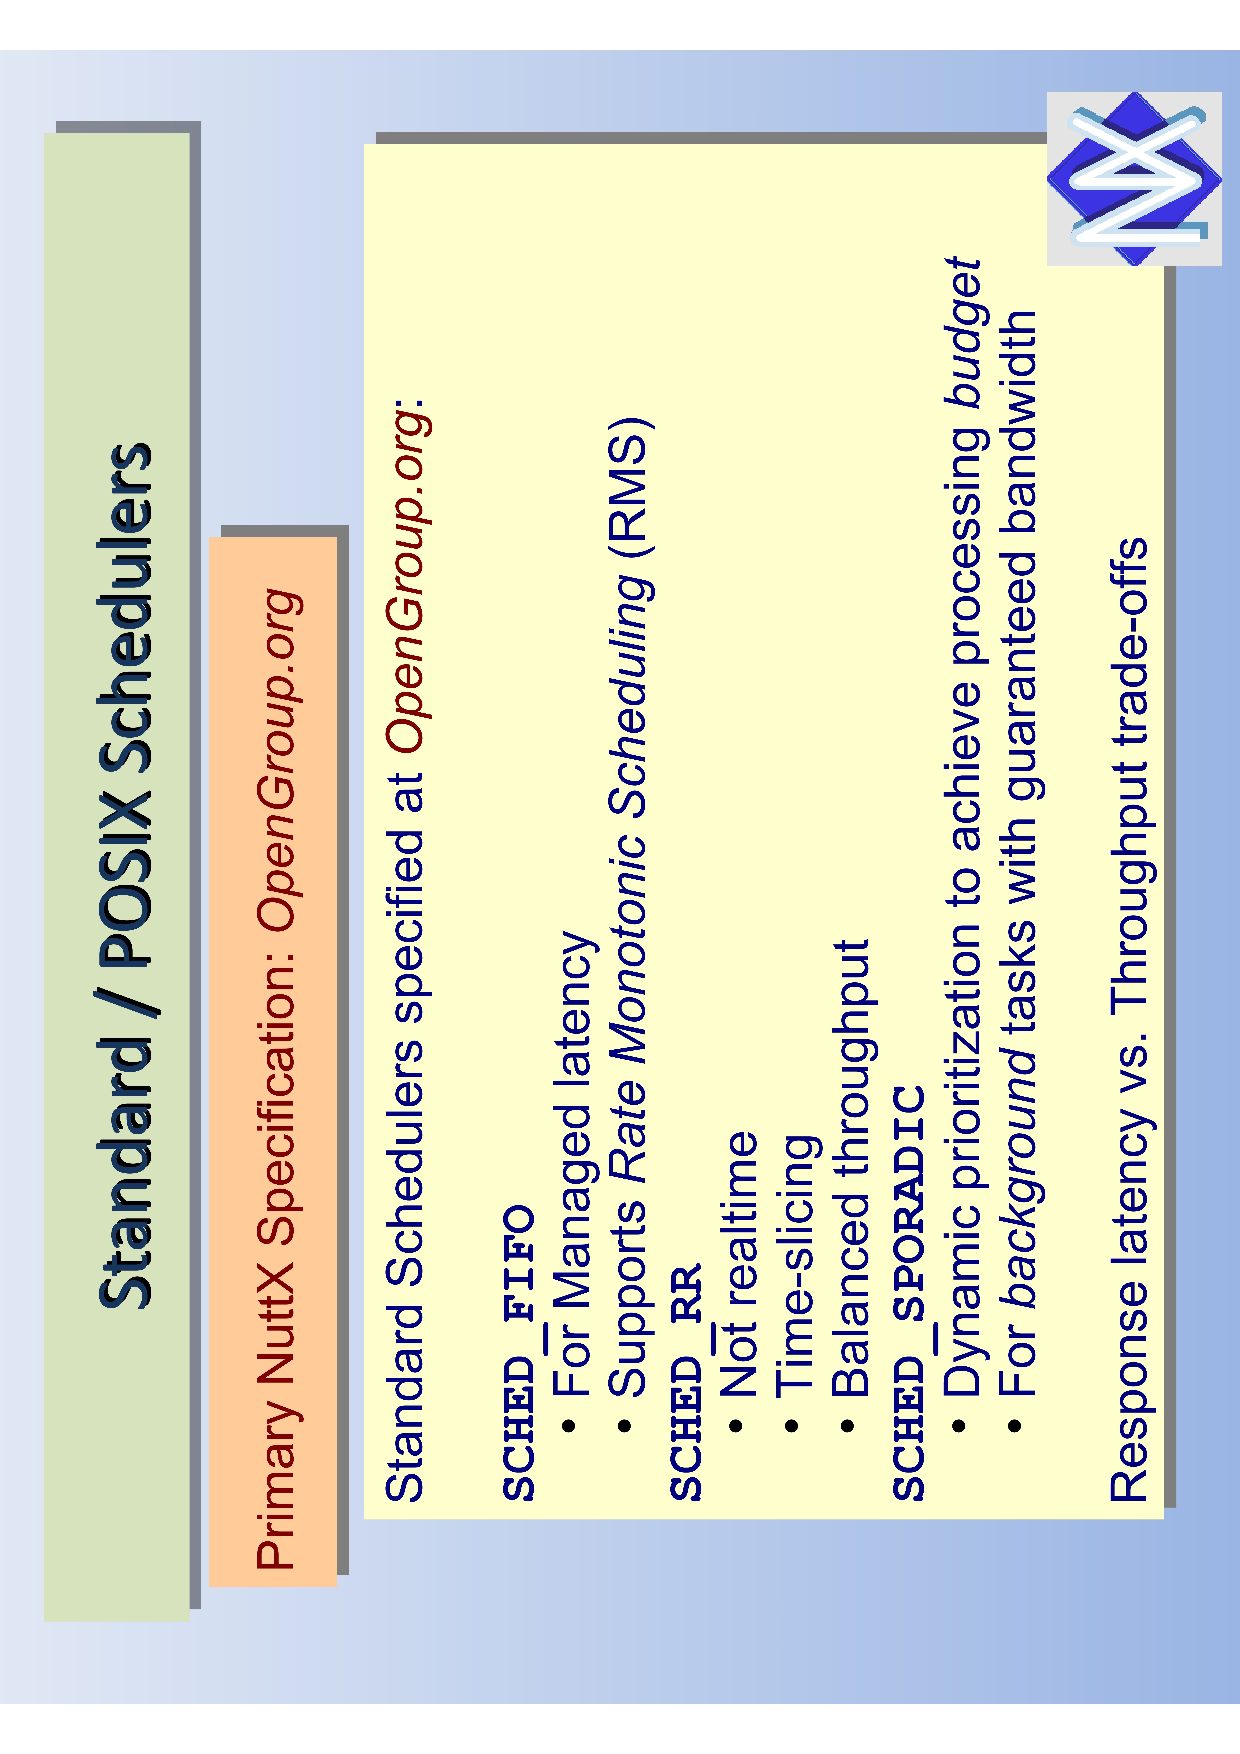
\includegraphics[angle=-90,origin=c,width=0.95\linewidth]{escalonadores.pdf}
	\onslide<2>\centering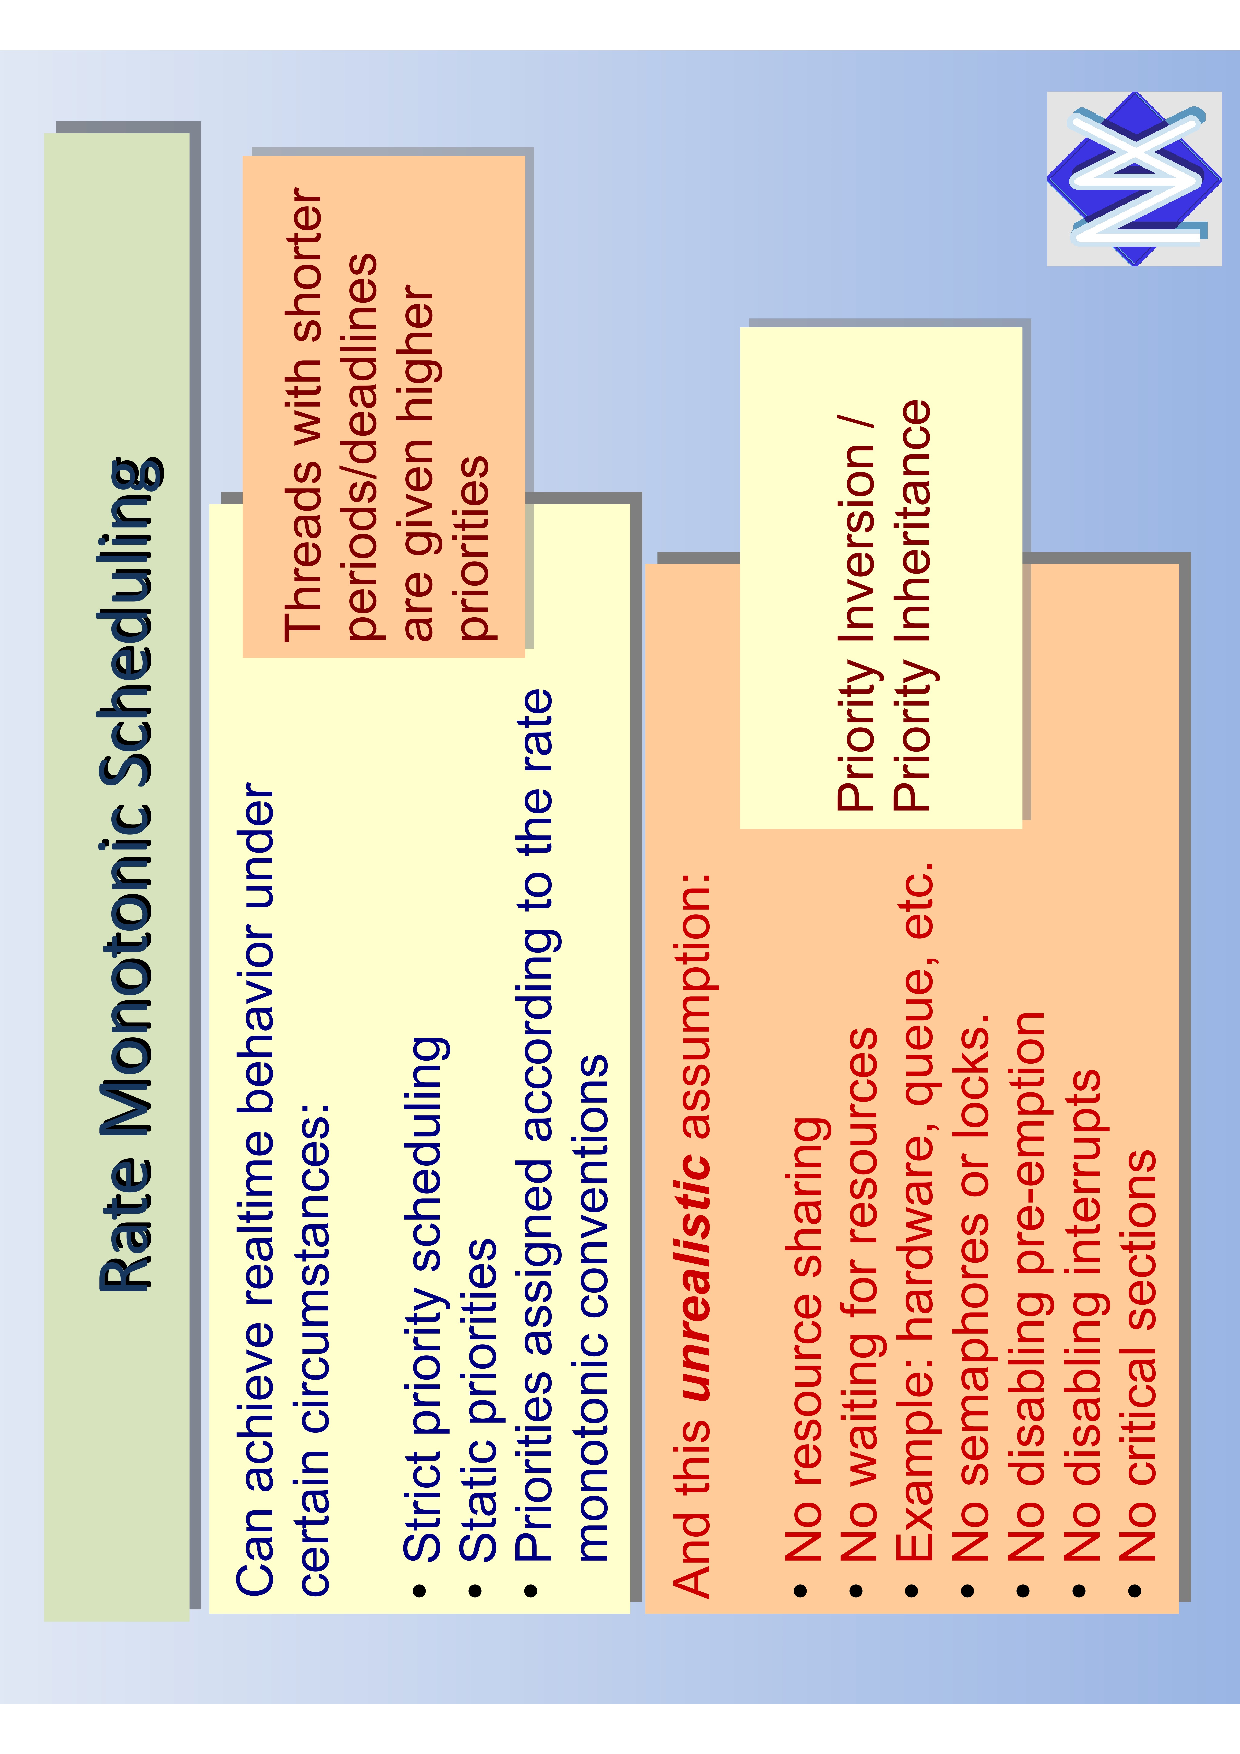
\includegraphics[angle=-90,origin=c,width=0.95\linewidth]{real.pdf}
	\onslide<3>\centering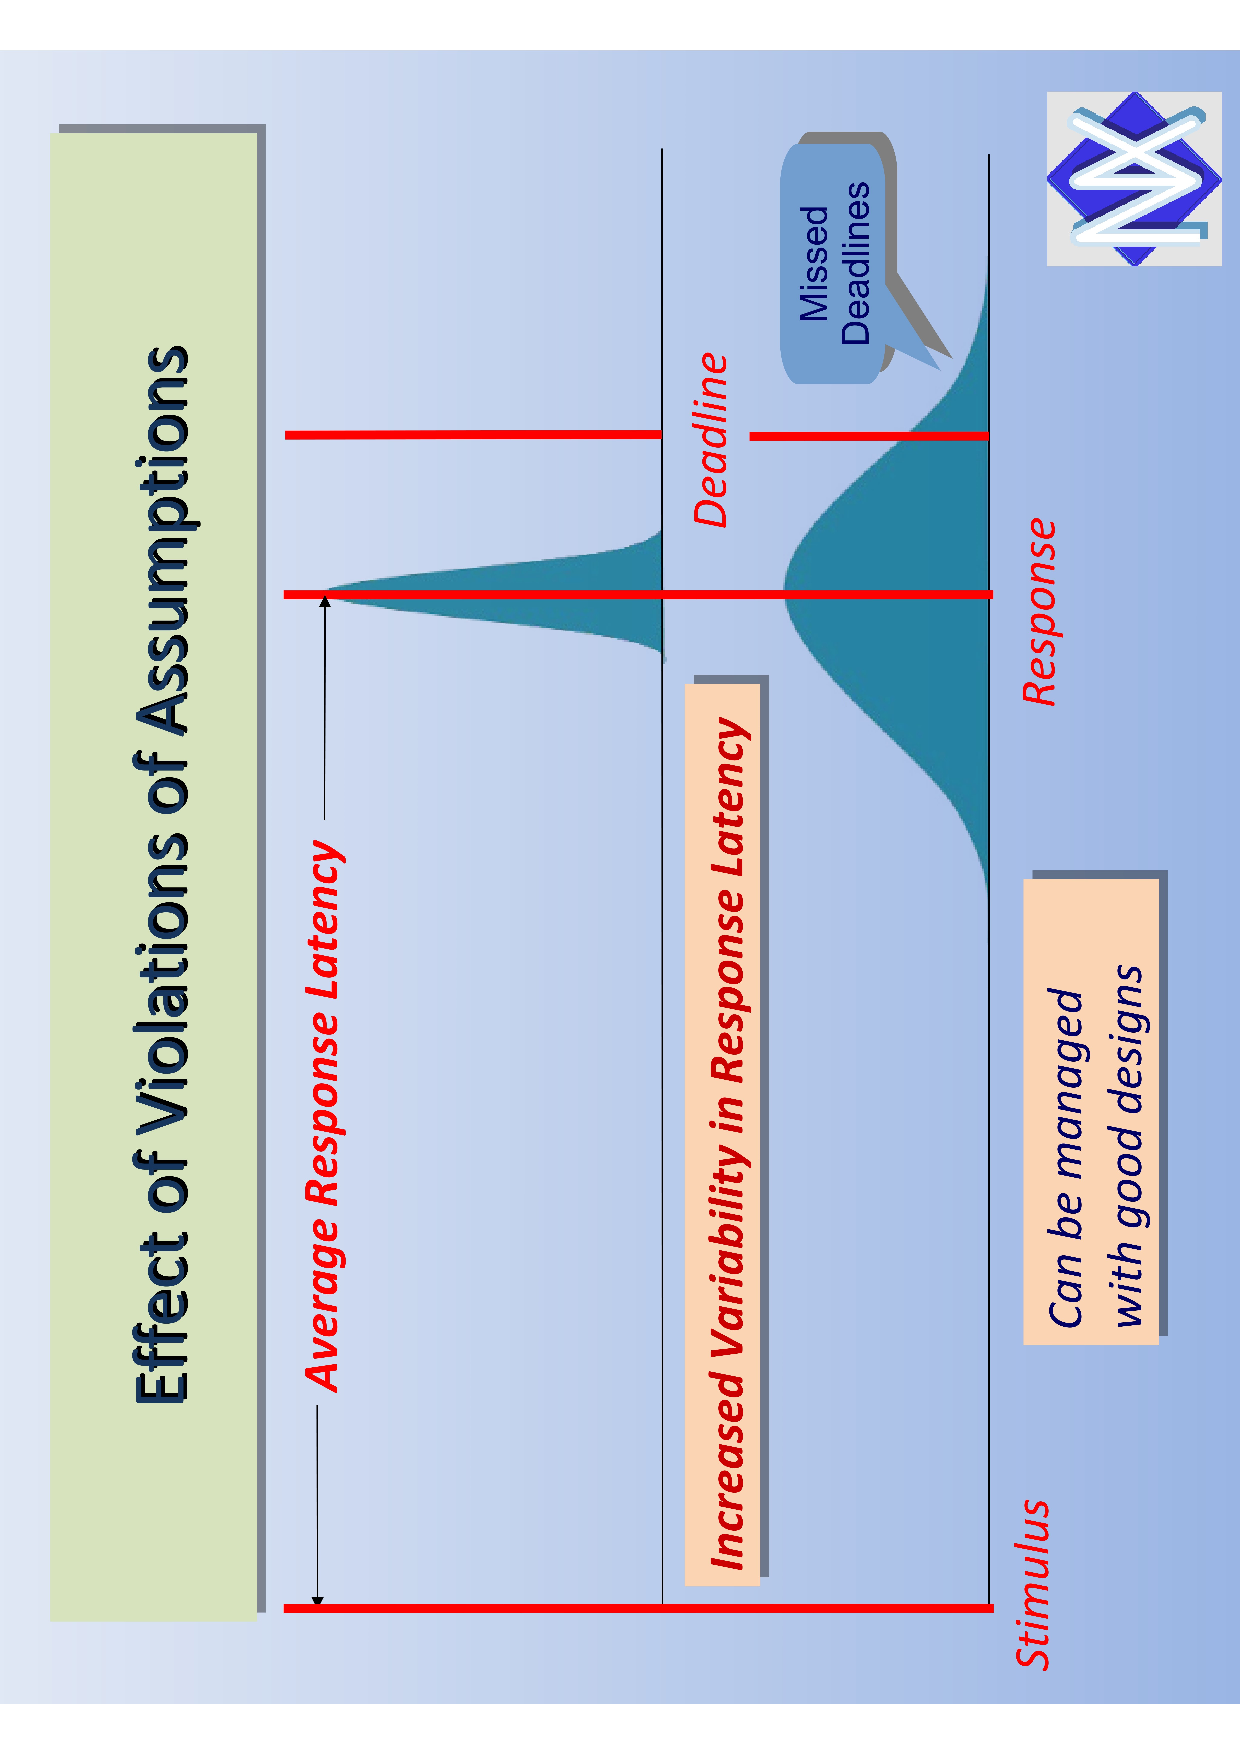
\includegraphics[angle=-90,origin=c,width=0.95\linewidth]{distribuição.pdf}
	\onslide<4>\centering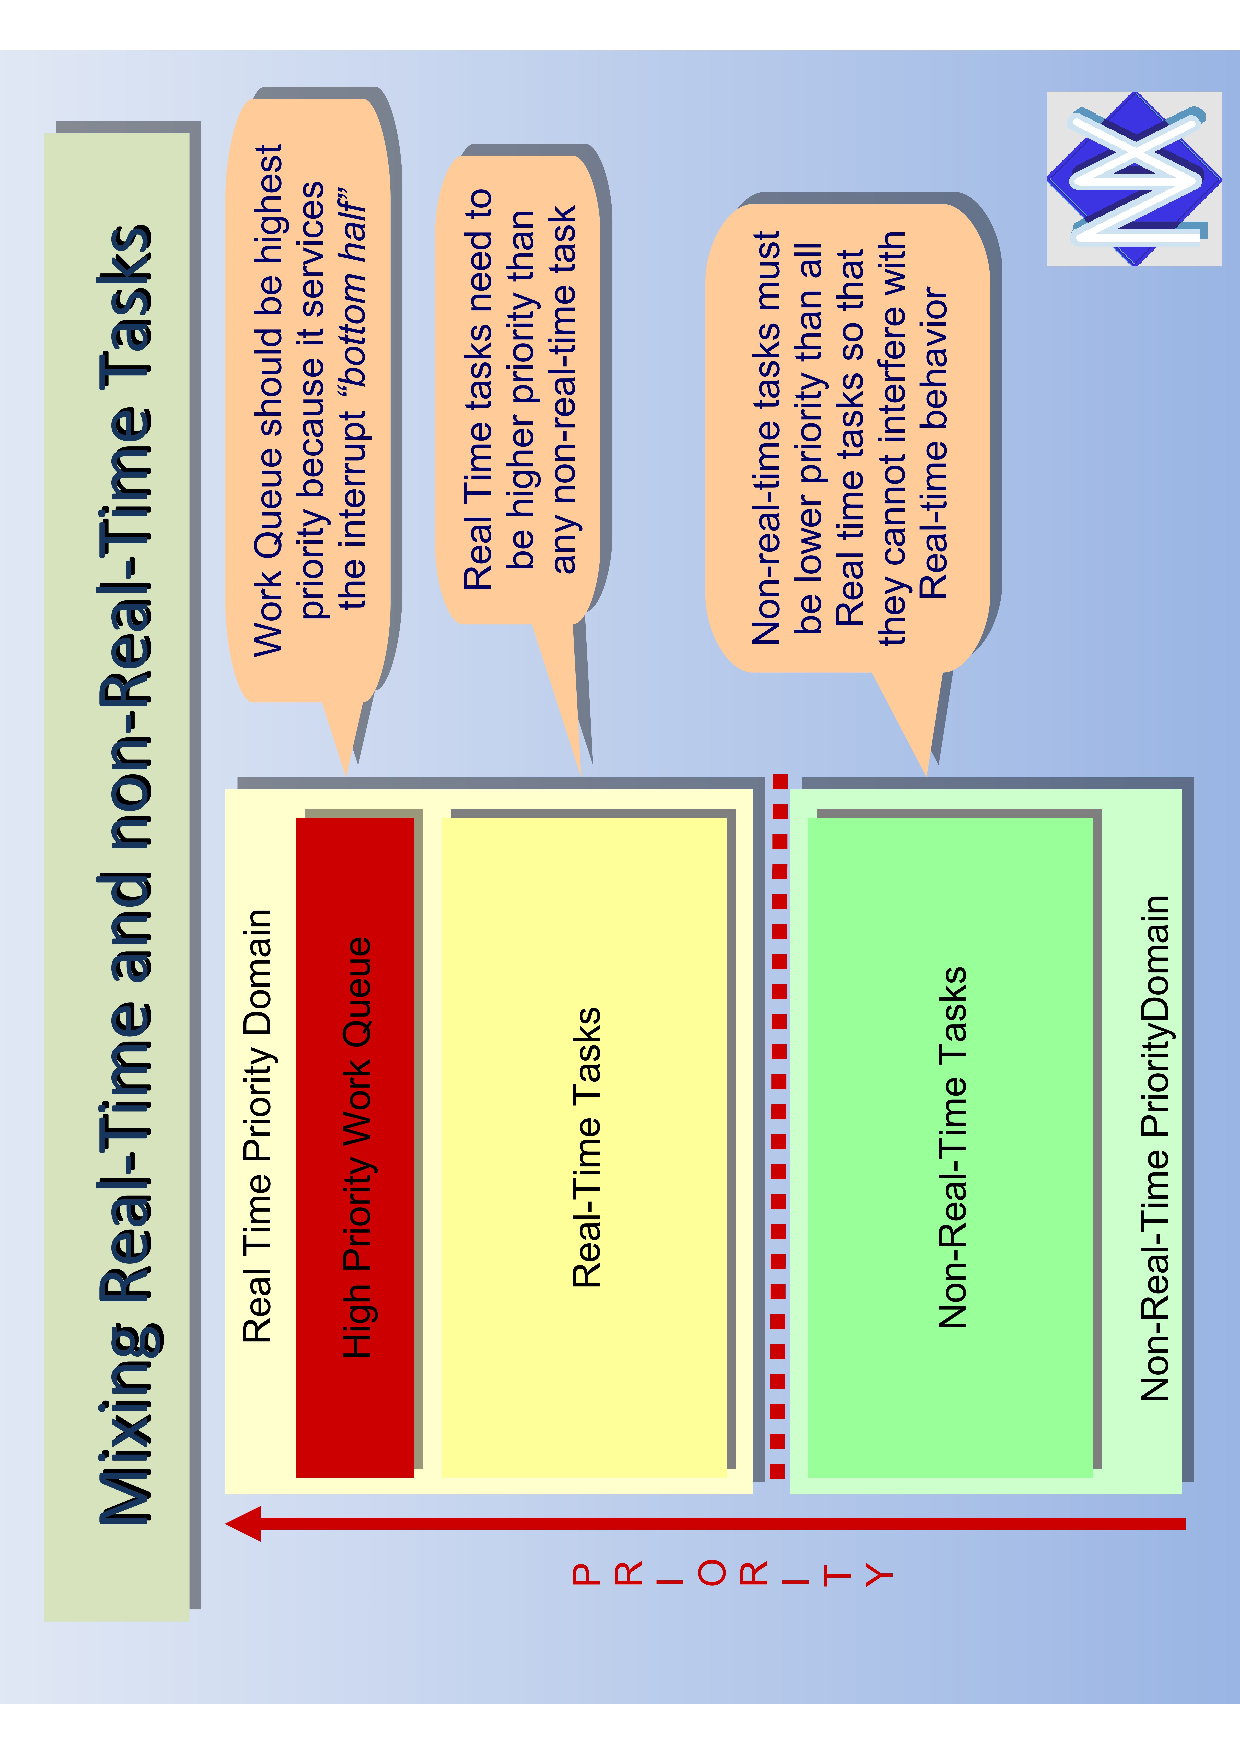
\includegraphics[angle=-90,origin=c,width=0.95\linewidth]{mistura.pdf}
  \end{overprint}
\end{minipage}

\end{frame}

% ----------------- NOVO SLIDE --------------------------------
\section{Aplicações}
\begin{frame}{Aplicações}

\begin{minipage}{0.5\textwidth}
  \begin{itemize}
    \justifying
    \item \visible<1->{O NuttX satisfaz requerimentos para aplicações que necessitam de um RTOS com utilitários compatíveis com POSIX, com ferramentas similares do BSD/Linux e com a biblioteca libc, porém com \textit{footprint} reduzido;}
    \item \visible<2->{Linha de produtos de áudio da SONY;}
    \item \visible<3->{Capas inteligentes do modelo Moto Z da Motorola (Snaps e Mods);}
  \end{itemize}
\end{minipage}%
\begin{minipage}{0.5\textwidth}
  \centering
  \begin{overprint}
  	\onslide<2>\centering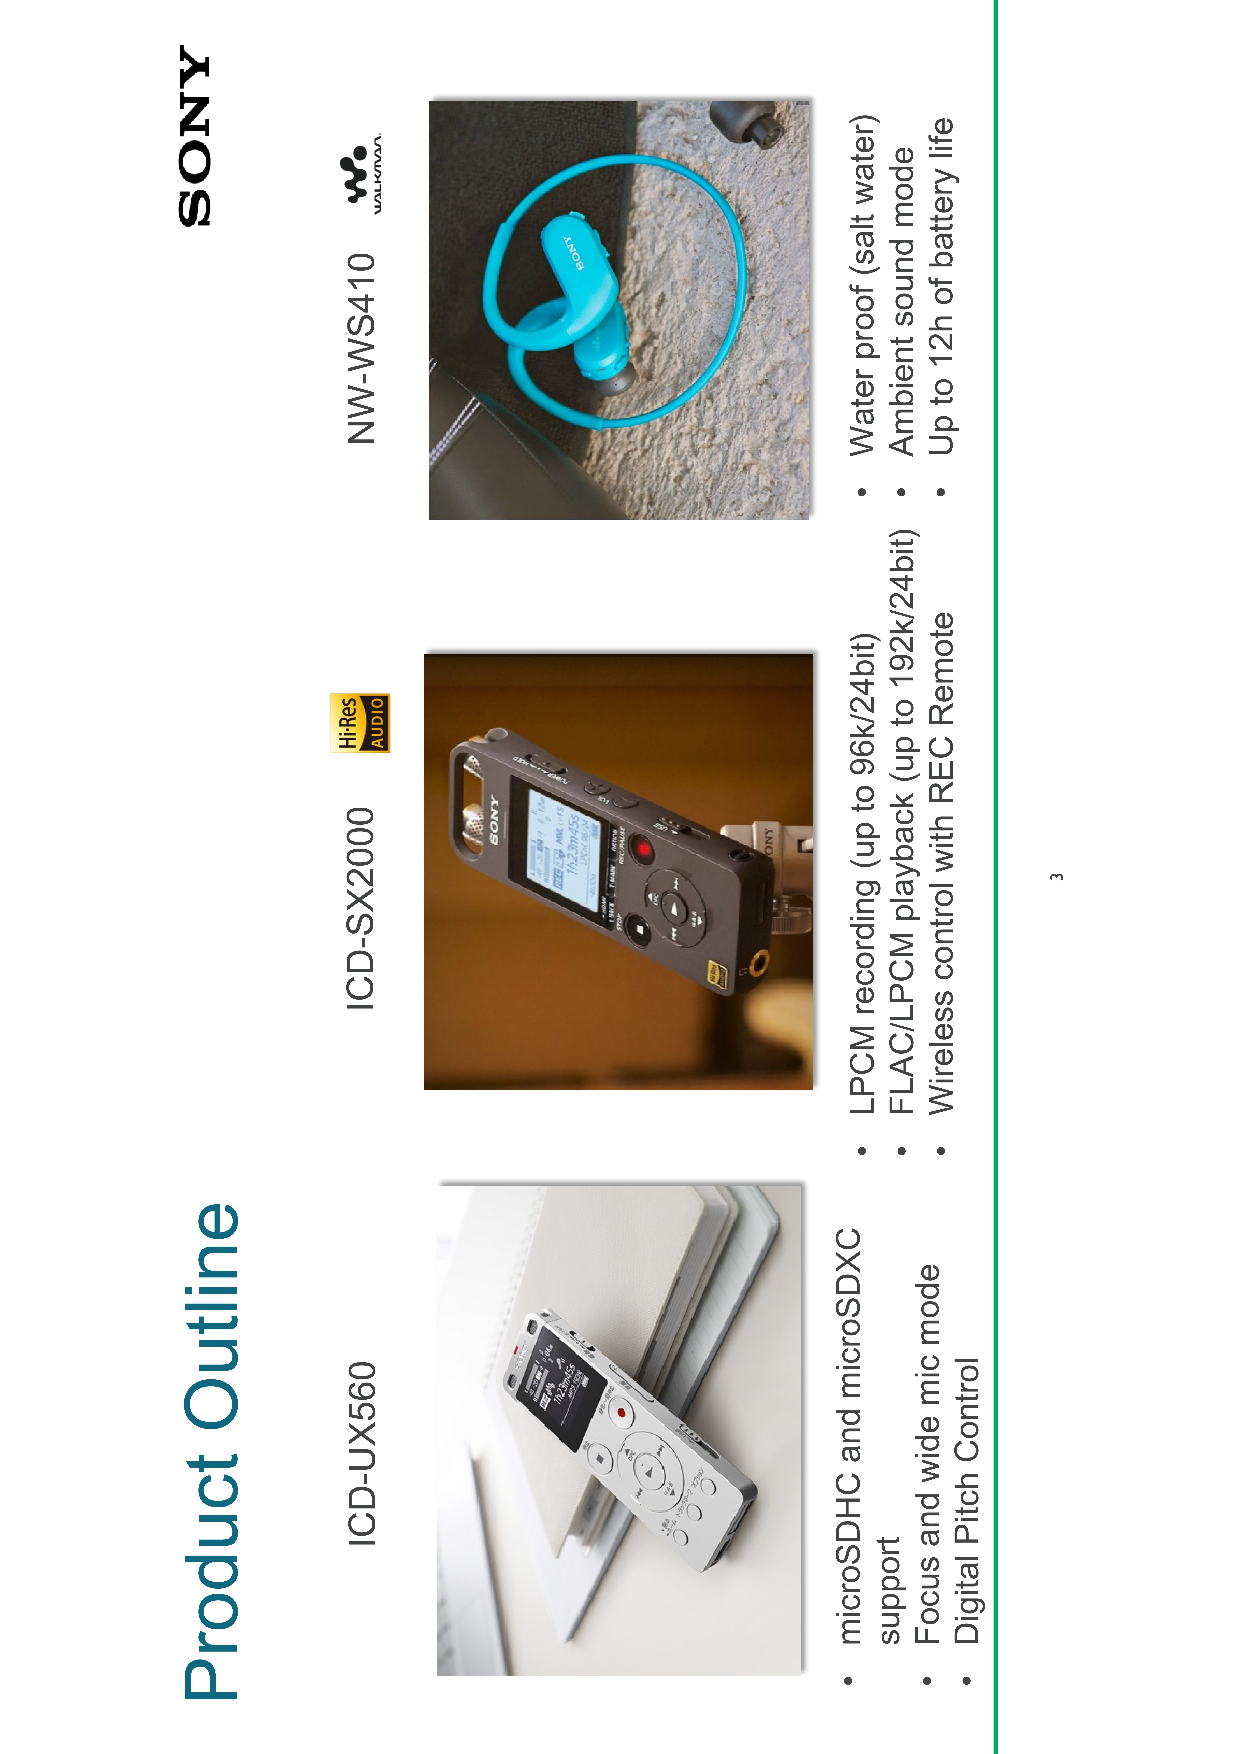
\includegraphics[angle=-90,origin=c,width=0.95\linewidth]{sony.pdf}
	\onslide<3>\centering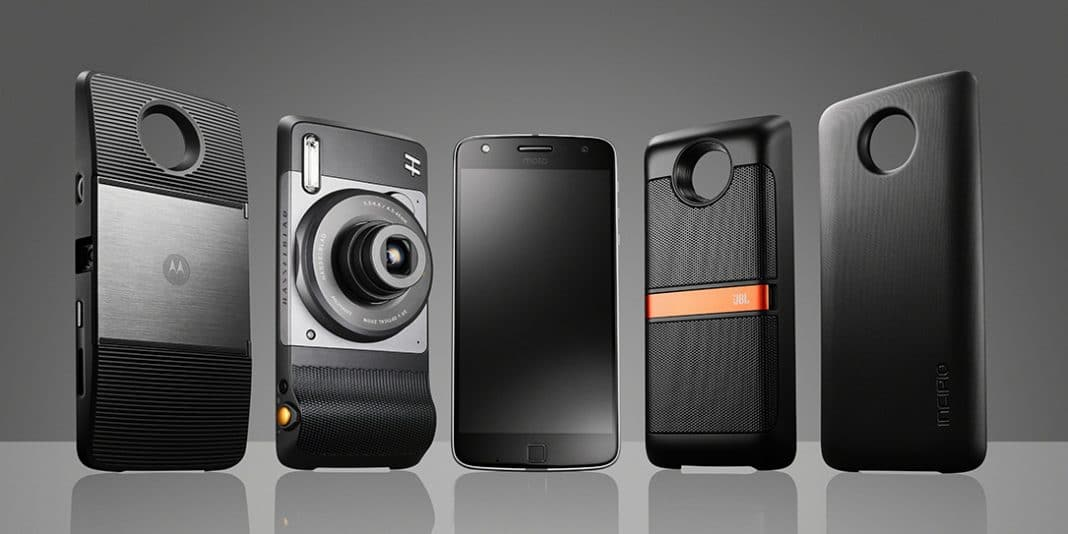
\includegraphics[width=0.95\linewidth]{moto.jpg}
  \end{overprint}
\end{minipage}

\end{frame}

% ----------------- NOVO SLIDE --------------------------------
\begin{frame}{Aplicações}

\begin{minipage}{0.5\textwidth}
  \begin{itemize}
    \justifying
    \item \visible<1->{Módulo Pixhawk 4 (PX4) de piloto automático de veículos aéreos não tripulados (drones) da 3DRobotics;}
    \item \visible<2->{Thingsee One, conjunto de sensores portátil com E/S cabeada e sem fio, também com HIDs e armazenamento expansível para testes de desenvolvedores, fabricado pela Haltian.}
  \end{itemize}
\end{minipage}%
\begin{minipage}{0.5\textwidth}
  \centering
  \begin{overprint}
	\onslide<1>\centering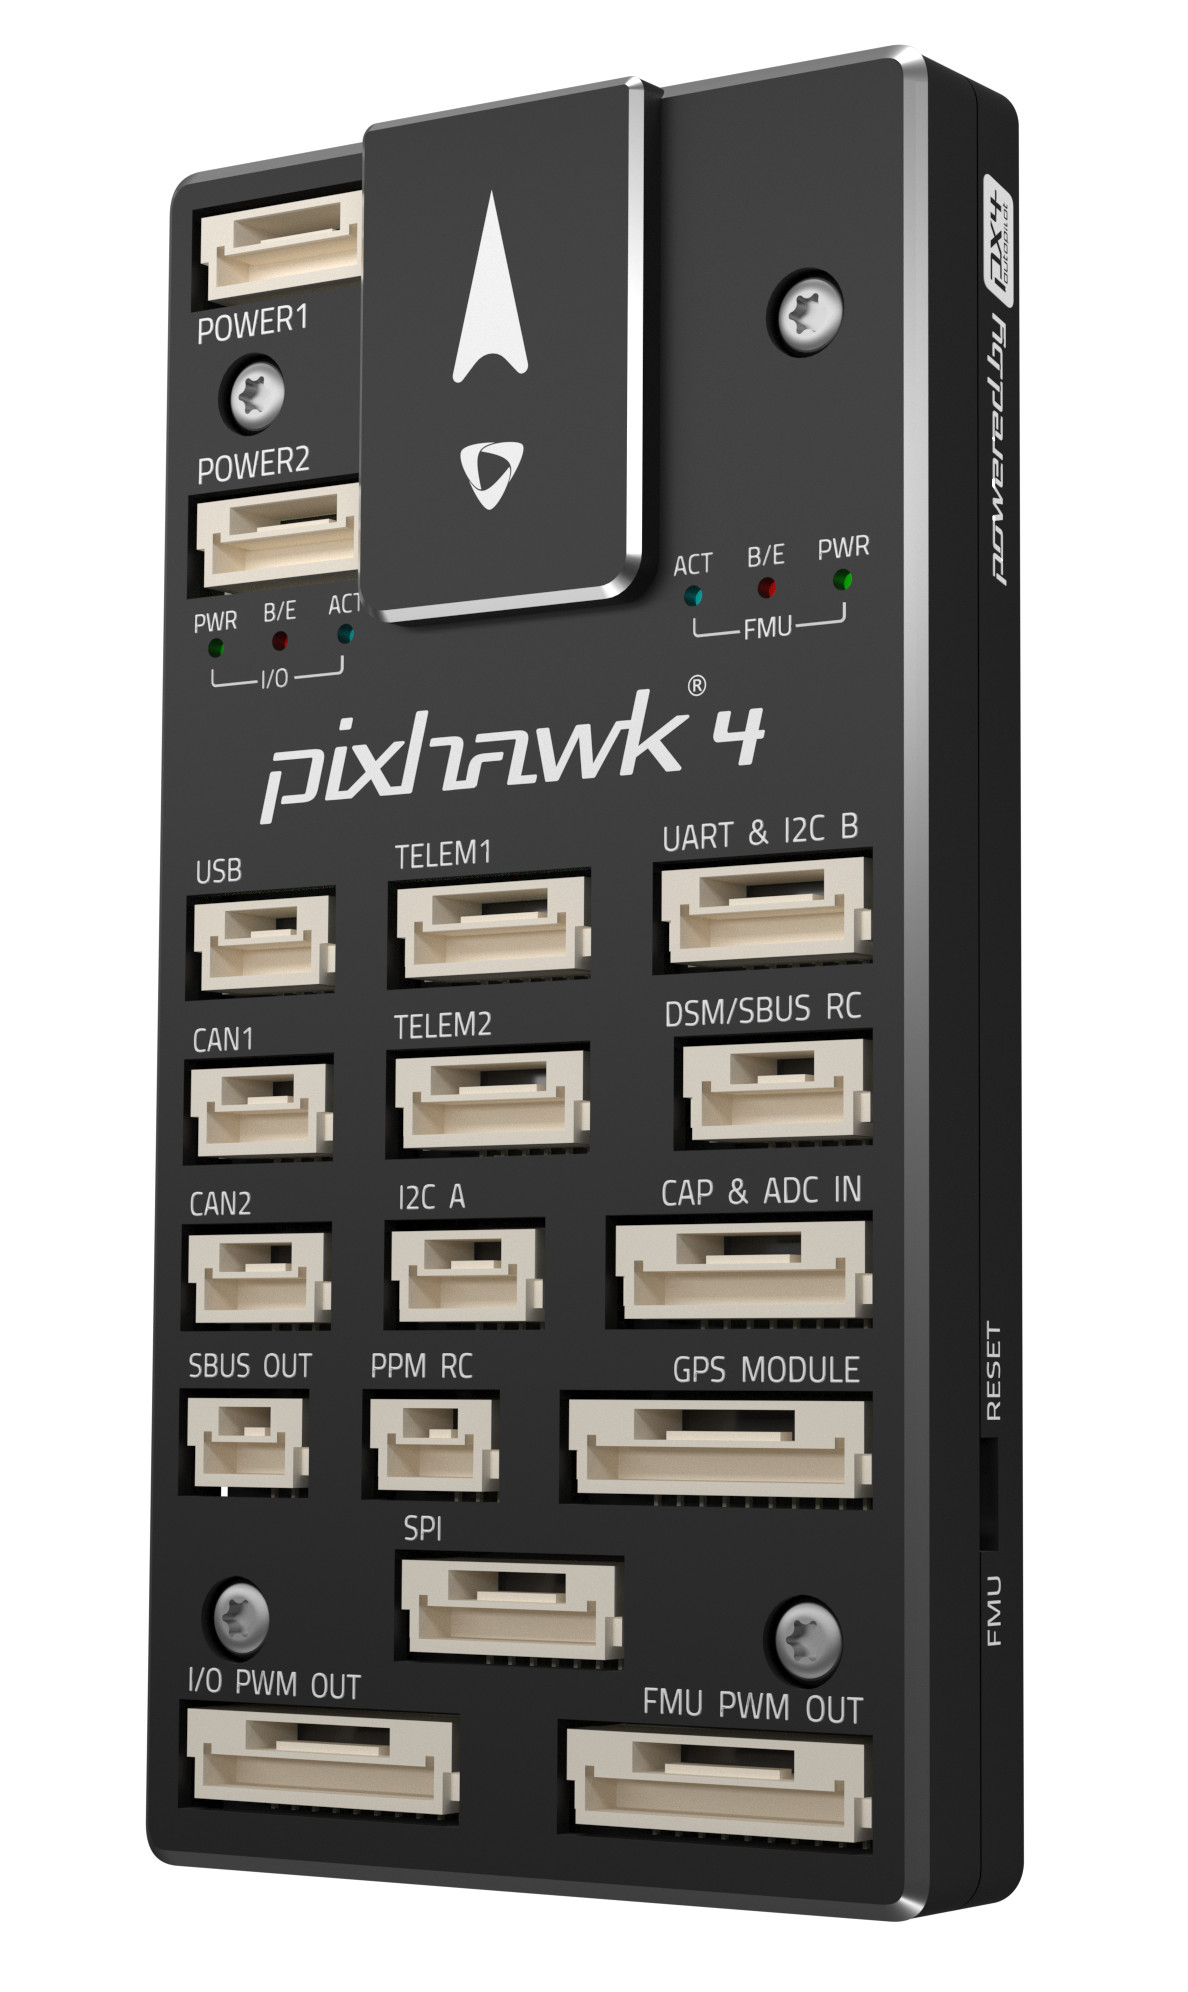
\includegraphics[width=0.60\linewidth]{px4.jpg}
	\onslide<2>\centering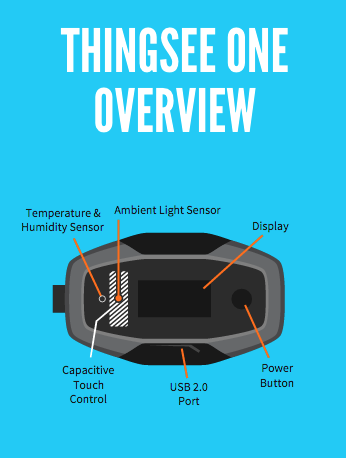
\includegraphics[width=0.70\linewidth]{thingsee.png}
  \end{overprint}
\end{minipage}

\end{frame}

% ----------------- NOVO SLIDE --------------------------------
\section{Conclusão}
\begin{frame}{Conclusão}

\begin{block}{Final da apresentação}
	Perguntas?
\end{block}

\end{frame}

% ----------------- NOVO SLIDE --------------------------------
\section{Referências}

% --- O comando \allowframebreaks ---
% Se o conteúdo não se encaixa em um quadro, a opção allowframebreaks instrui 
% beamer para quebrá-lo automaticamente entre dois ou mais quadros,
% mantendo o frametitle do primeiro quadro (dado como argumento) e acrescentando 
% um número romano ou algo parecido na continuação.

\begin{frame}[allowframebreaks]{Referências}
\bibliography{referencias}
\end{frame}

% ----------------- FIM DO DOCUMENTO -----------------------------------------
\end{document}
